\documentclass[review]{elsarticle}

\usepackage{lineno,hyperref}
\modulolinenumbers[5]
\usepackage{booktabs}
\usepackage{graphicx}
\usepackage{float}
\graphicspath{ {./images/} }
\usepackage{adjustbox}

\usepackage{threeparttable}
\usepackage{amsmath}
\usepackage[font=small,skip=0pt]{caption}

\journal{International Journal of Forecasting}

%%%%%%%%%%%%%%%%%%%%%%%
%% Elsevier bibliography styles
%%%%%%%%%%%%%%%%%%%%%%%
%% To change the style, put a % in front of the second line of the current style and
%% remove the % from the second line of the style you would like to use.
%%%%%%%%%%%%%%%%%%%%%%%

%% Numbered
%\bibliographystyle{model1-num-names}

%% Numbered without titles
%\bibliographystyle{model1a-num-names}

%% Harvard
%\bibliographystyle{model2-names.bst}\biboptions{authoryear}

%% Vancouver numbered
%\usepackage{numcompress}\bibliographystyle{model3-num-names}

%% Vancouver name/year
%\usepackage{numcompress}\bibliographystyle{model4-names}\biboptions{authoryear}

%% APA style
%\bibliographystyle{model5-names}\biboptions{authoryear}

%% AMA style
%\usepackage{numcompress}\bibliographystyle{model6-num-names}

%% `Elsevier LaTeX' style
\bibliographystyle{elsarticle-num}
%%%%%%%%%%%%%%%%%%%%%%%

\begin{document}

  \begin{frontmatter}

    \title{A novel interval electricity prices forecasting using Residual Neural Networks (ResNet)}
    % \tnotetext[mytitlenote]{Fully documented templates are available in the elsarticle package on \href{http://www.ctan.org/tex-archive/macros/latex/contrib/elsarticle}{CTAN}.}

    %% Group authors per affiliation:
    % \author{Pornchai Chaweewat\fnref{myfootnote}}
    \author{Pornchai Chaweewat\fnref{myfootnote}}
    \author{Jai Govind Singh\fnref{myfootnote2}}

    \address{Department of Energy, Environmental and Climate Change, School of Environmental, Resource and Development, Asian Institute of Thechnology, Thailand}
    \fntext[myfootnote]{email: chaweewat.p@gmail.com}
    \fntext[myfootnote2]{email: jgsingj@ait.ac.th}

    % %% or include affiliations in footnotes:
    % \author[mymainaddress,mysecondaryaddress]{Elsevier Inc}
    % \ead[url]{www.elsevier.com}
    %
    % \author[mysecondaryaddress]{Global Customer Service\corref{mycorrespondingauthor}}
    % \cortext[mycorrespondingauthor]{Corresponding author}
    % \ead{support@elsevier.com}
    %
    % \address[mymainaddress]{1600 John F Kennedy Boulevard, Philadelphia}
    % \address[mysecondaryaddress]{360 Park Avenue South, New York}

    \begin{abstract}
      This paper proposed a novel electricity prices forecasting method based on a novel Residual Neural Network (ResNet) for probabilistic electricity prices forecasting.
      A proposed new model was developed from a ResNet approach which is capable of spike prices and interval prices value forecasting.
      The proposed ResNet was consisting of two network layers.
      The first neural network layers were probabilistic spike prices prediction part.
      The output of second neural network layers was formulated to interval prices forecasting by Lower and Upper Bound Estimation (LUBE) methods.
      The LUBE methods included quantile regression (QR) and Mean and Variance (MV) estimation.
      The proposed forecasting models were demonstrated with GEFCom2014 dataset.
      The dataset was consisting of 15 tasks for electricity prices forecasting.
      The results were compared with GEFCom2014's benchmarks, Quantile Regression Average (QRA) and Multilayer Perceptron Network (MLP) approaches.
      The performances of forecasting models were evaluated in term of accuracy and reliability metrics by Pinball Loss Function and Coverage Width-based Criterion (CWC), respectively.
      The significant outcome of this paper was that the forecasting model, ResNet, cooperated with spike prices prediction improved the forecasting's performance in term of accuracy and reliability aspects.
      Moreover, increasing in confidence level could generate lower CWC values and represent high reliability's satisfaction.
    \end{abstract}

    \begin{keyword}
      electricity prices, interval forecasting, multilayer perceptron, LUBE, quantile regression, mean and variance estimation, pinball loss function, coverage width-based criterion, GEFCom2014
    \end{keyword}

  \end{frontmatter}

  \linenumbers

  \section{Introduction}

    Since the transformation of the deregulation of modern power systems, electricity prices forecasting has become a more critical process to energy market's participants at planning and operation levels.
    As a result of a higher number of fluctuated electricity prices as well as the number of unanticipated spike prices occurrences, the occurrences of spike prices can cause financial damage to both customers and producers.
    The sudden lack of available generations or disconnected of transmission lines exponentially accelerates of electricity prices volatility and causes either very high and spike prices.
    The spike prices can reach several times to thousand times of the regular price.
    In different circumstances, negative prices occur when there is an excess of renewable generation.
    Several pieces of evidence show that the spike prices are around 100$\$$/MWhr may result from usual congestion or unexpected overload, while spiking prices around $\$$500/MWhr led by lacking reserve.

    \cite{He2016} proposed that insufficient reserves influence the spike price in the day ahead clearing market.
    On the other hand, real-time spike price is influenced by the outage or interrupted of the generation or transmission system.
    It can cause higher than $\$$1,000/MWhr in electricity price.

    \cite{SINGHAL2011550} provided fundamental reasons for spike prices which are volatility of fuel price, load uncertainty, fluctuation in hydroelectricity production, generation outage, transmission congestion, a behavior of market participation and market manipulation.
    \cite{GONZALEZSOTRES2017338} studied on technique and economical of on centralized voltage control with high PV penetration in Portuguese network.
    These results illustrated that improvement in both forecasting tools and communication systems have a significant impact on dedicate resources and voltage control.


    In works of literature, over the past few decades, many powerful forecasting algorithms have been developed (for a recent comprehensive review, see \cite{Weron2014}).
    The commonly forecast electricity prices models are classified into two primary categories; time-series models and soft computing models which is non-time series models.
    The regular time-series model have been habitually applied to electricity price forecasting model.
    Examples of time-series forecasgting models are autoregressive integrated moving average (ARIMA)\cite{1216141}, Autoregressive Moving Average eXogenous (ARMAX)\cite{7917305} and generalized autoregressive conditional heteroscedasticity (GARCH)\cite{4344162},\cite{1627232},
    The hybrid time-series models were proposed such as autoregressive-GARCH\cite{Girish2016} and wavelet-ARIMA\cite{1425601}.

    Despite the time-series model, in recent pieces of literature, the concept of applying of artificial neural network (ANN) in forecast future electricity prices was proposed in \cite{Catalao2007}.
    Recently, electricity prices forecasting based deep neural network was developed in \cite{Kuo2018}.
    The hybrid ANN models were proposed such as ANN-ABC\cite{Chaweewat2017}, wavelet-ANN\cite{Bento2018}, and wavelet-SOM-ANN\cite{NAZAR2018214}.
    The result of previous electricity prices forecasting studies shows that the electricity prices forecasting based on the ANN model performed better than time-series models, such as ARIMA models \cite{Keles2016}.
    The electricity prices are frequently changed and not in a weekly pattern as a result of the problem in time-series techniques (AR, ARIMA, GARCH)\cite{4077090}.

    The majority of empirical studies was on point forecasting (or call expected value of the spot price).
    The general point predictions produced no information about sampling errors and prediction accuracy.
    This lead to confidence intervals (CIs) and prediction intervals (PIs) \cite{Weron2014}.
    CIs and PIs were two favorite tools for quantifying and representing the uncertainty of predictions.
    Consequently, the use of prediction interval or probabilistic forecasting was interested due to it help market participants to submit effective bids with low risks.
    In literature, several methods have been proposed for construction of PIs and CIs assessment.
    Lower Upper Bounds Estimation (LUBE) method was formulated using mean and variance estimation which was proposed in \cite{Khosravi2011}.
    Besides, delta technique for PI construction was presented in \cite{KhosraviA2010}.

    % (mention on used of deep residual neural network and why we use this method)
    In computational intelligent area, Residual neural network (ResNet) was widely used in computer vision and pattern recognition \cite{DBLP:journals/corr/HeZRS15}, \cite{DBLP:journals/corr/ZagoruykoK16}.
    ResNet was modified from deep Feed Forward Neural Networks (FFNNs) with extra connections (or called skip connections). The input is passing from one layer to a late layer as well as the next layer as shown in Figure~\ref{Fig:Basic_DRNN}.
    However, there were no used of ResNet in forecasting applications.

    \begin{figure}[H]
      \centering
      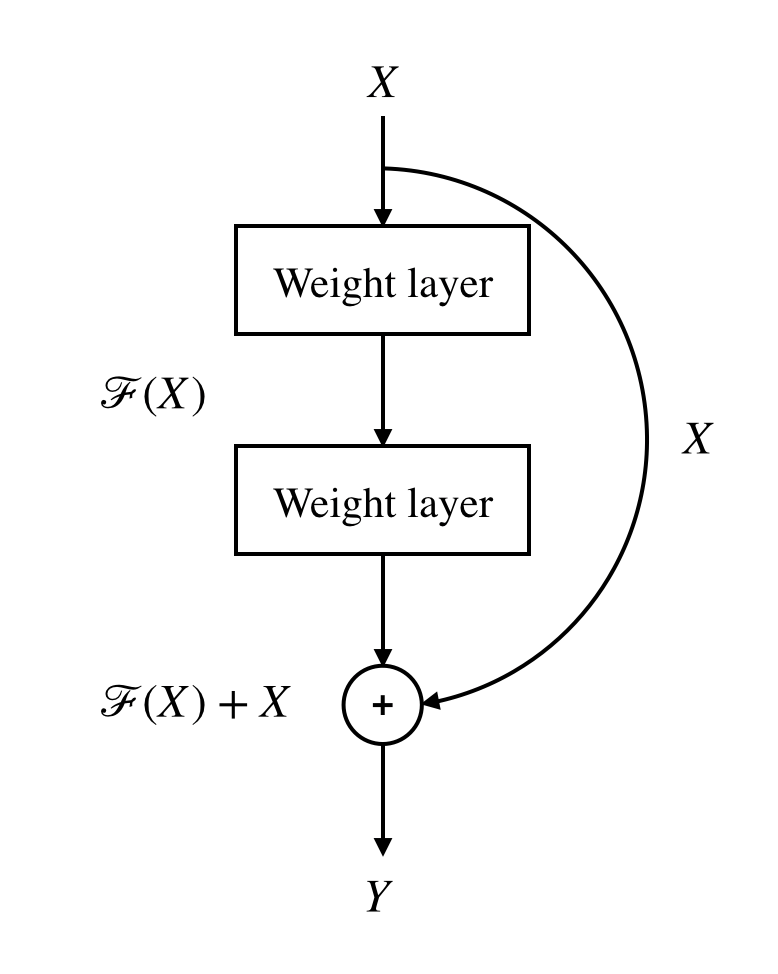
\includegraphics[width=5cm]{basic_DRNN}
      \caption{Basis concept of Residual Neural Network (ResNet).}
      \label{Fig:Basic_DRNN}
    \end{figure}

    % (proposal)
    Therefore, this paper seeks to utilize ResNet in electricity prices forecasting.
    The performance results of the ResNet forecasting model were compared with quantile regression average (QRA) \cite{Maciejowska2016} and MLP techniques.

    The novelty of this study is twofold.
    First, ResNet is first used in the field of probabilistic electricity prices forecasting. As a result of the ResNet forecasting model, the probabilistic electricity prices forecasting can satisfy both accuracy and reliability aspects.
    Second, the use of Coverage Width-based Criterion (CWC) value evaluates interval electricity prices forecasting. The CWC value tests efficiency of forecasting model in term of reliability point of view.

    % (structure)
    The remainder of the paper is organized as follows.
    First, the problem formulation is presented in brief in section 2.
    Then, the central concept of the ResNet with LUBE algorithm in interval forecasting model is described.
    Next, the results after prediction processes of different tasks of proposed forecasting models are discussed in section 3.
    Finally, conclusions are drawn in the last section of this paper.

  \section{Problem formulation}
    This section will descript the construction of two proposed forecasting models; Multilayer Perceptron (MLP) and Residual Neural Network (ResNet) model.
    The MPL model will represent electricity prices forecasting without spike prices prediction (see related work in \cite{Dudek2016}), and the ResNet model will represent electricity prices forecasting with spike prices prediction within the model.
    Both models will generate upper and lower bounds concerning given confidence levels (5$\%$, 10$\%$, 15$\%$, 20$\%$, and 25$\%$).
    The upper and lower bound will be generated using quantile regression and mean and variance estimation method.

    \subsection{Proposed ResNet on interval prices forecasting}
      Here is a description of the structure of a proposed ResNet for interval electricity prices forecasting.
      As mention earlier, ResNet is constructed with plain layers and skip connections or called 'short-cut' to jump over some layers.
      The plain layers in this study consisted of probability spike prices layers and prices value layers.
      Firure~\ref{Fig:proposed_ResNet} illustrates a proposed novel ResNet for interval electricity prices forecasting.
      \begin{figure}[H]
        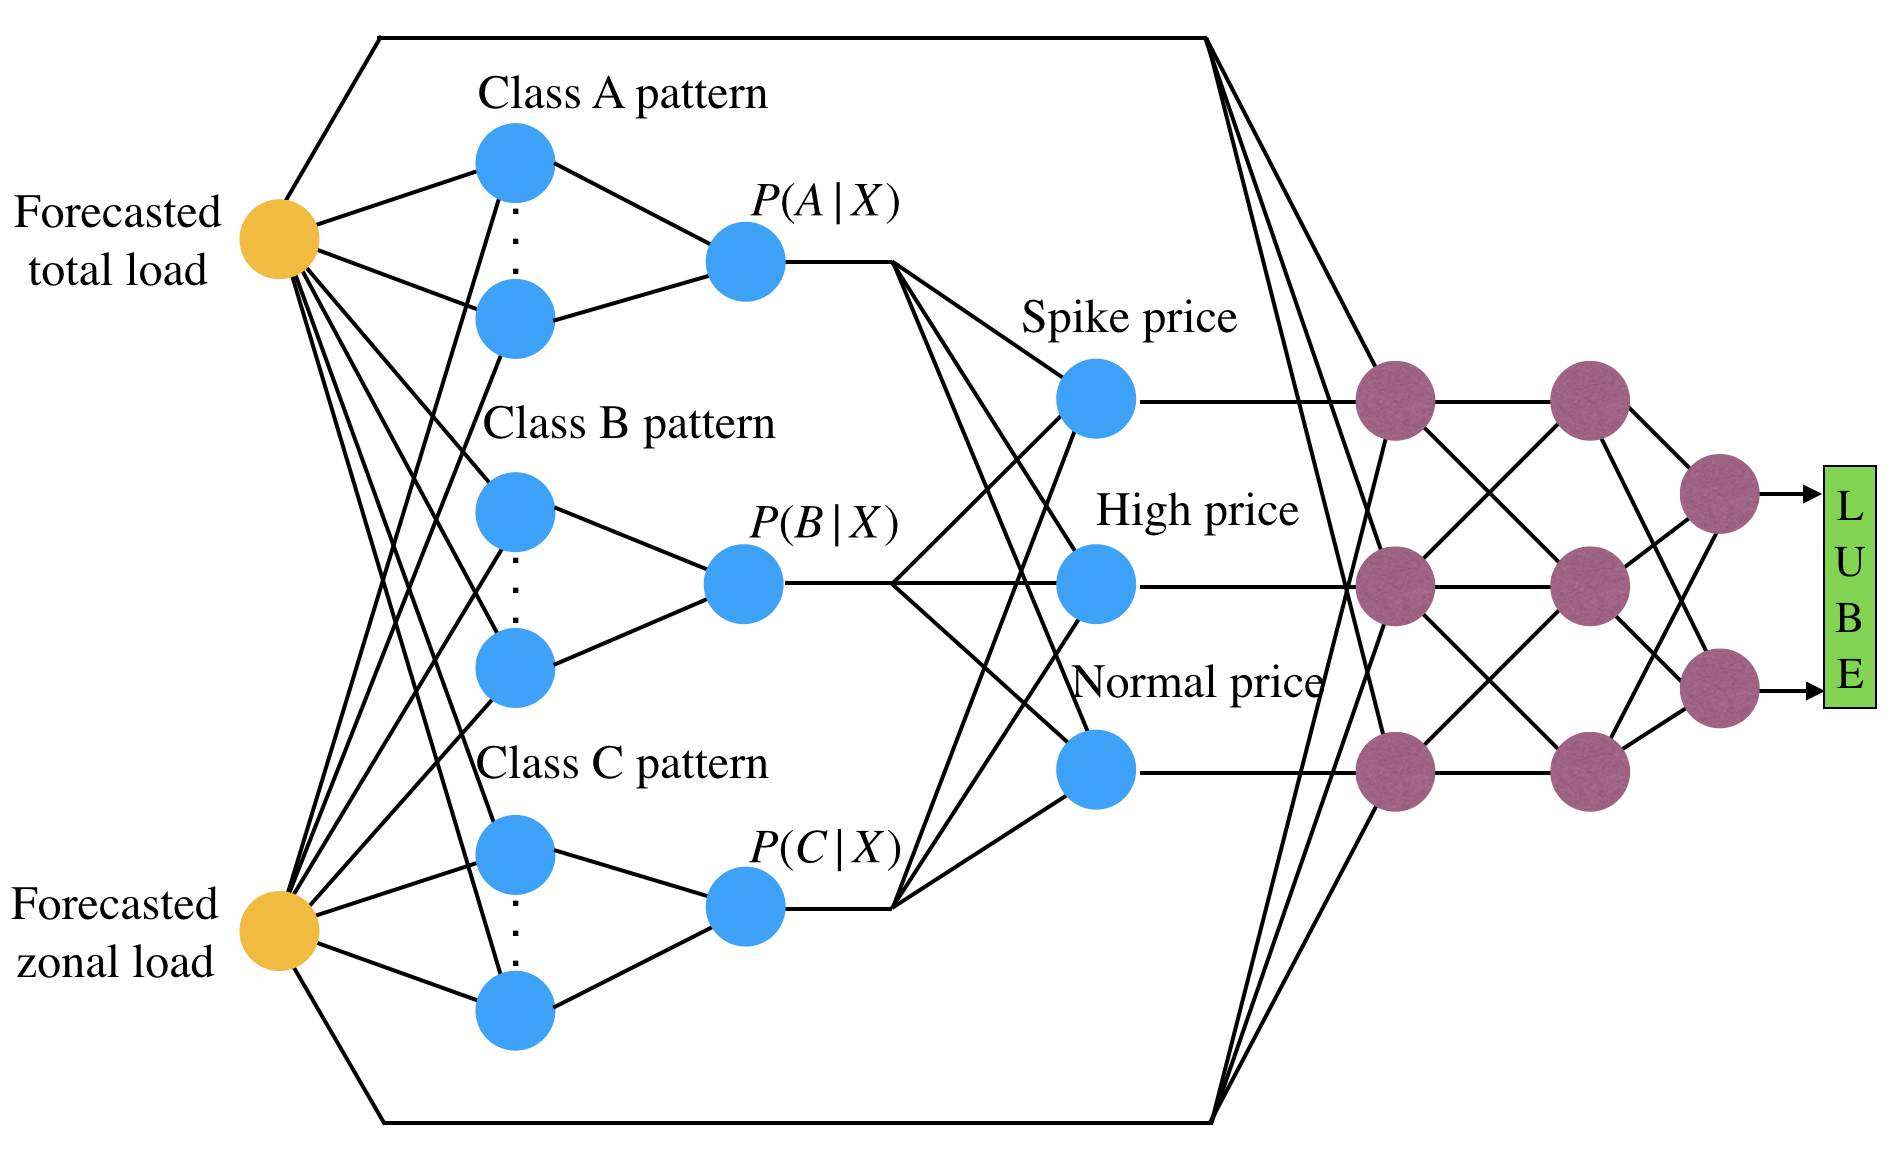
\includegraphics[width=12cm]{proposed_PDRNN}
        \caption{A proposed novel ResNet for interval electricity prices forecasting application.}
        \label{Fig:proposed_ResNet}
        \centering
      \end{figure}
      The input data forecasted system load and forecasted zonal load data, are fed to probabilistic spike prices layer, and prices value layer.
      The output of probability spike prices layer is regular, high and spike prices probabilistic value $P(A|X)$, $P(B|X)$, $P(C|X)$ at a set of given load values, $X$, respectively.
      Then, it multiplies with the fed input value to become inputs of prices value layers.
      The result of the ResNet is two values of forecasted upper and lower bound ($U_{i}$, $L_{i}$)of electricity prices at hour $i$ which will be descript in the next section.

      \begin{figure}[H]
        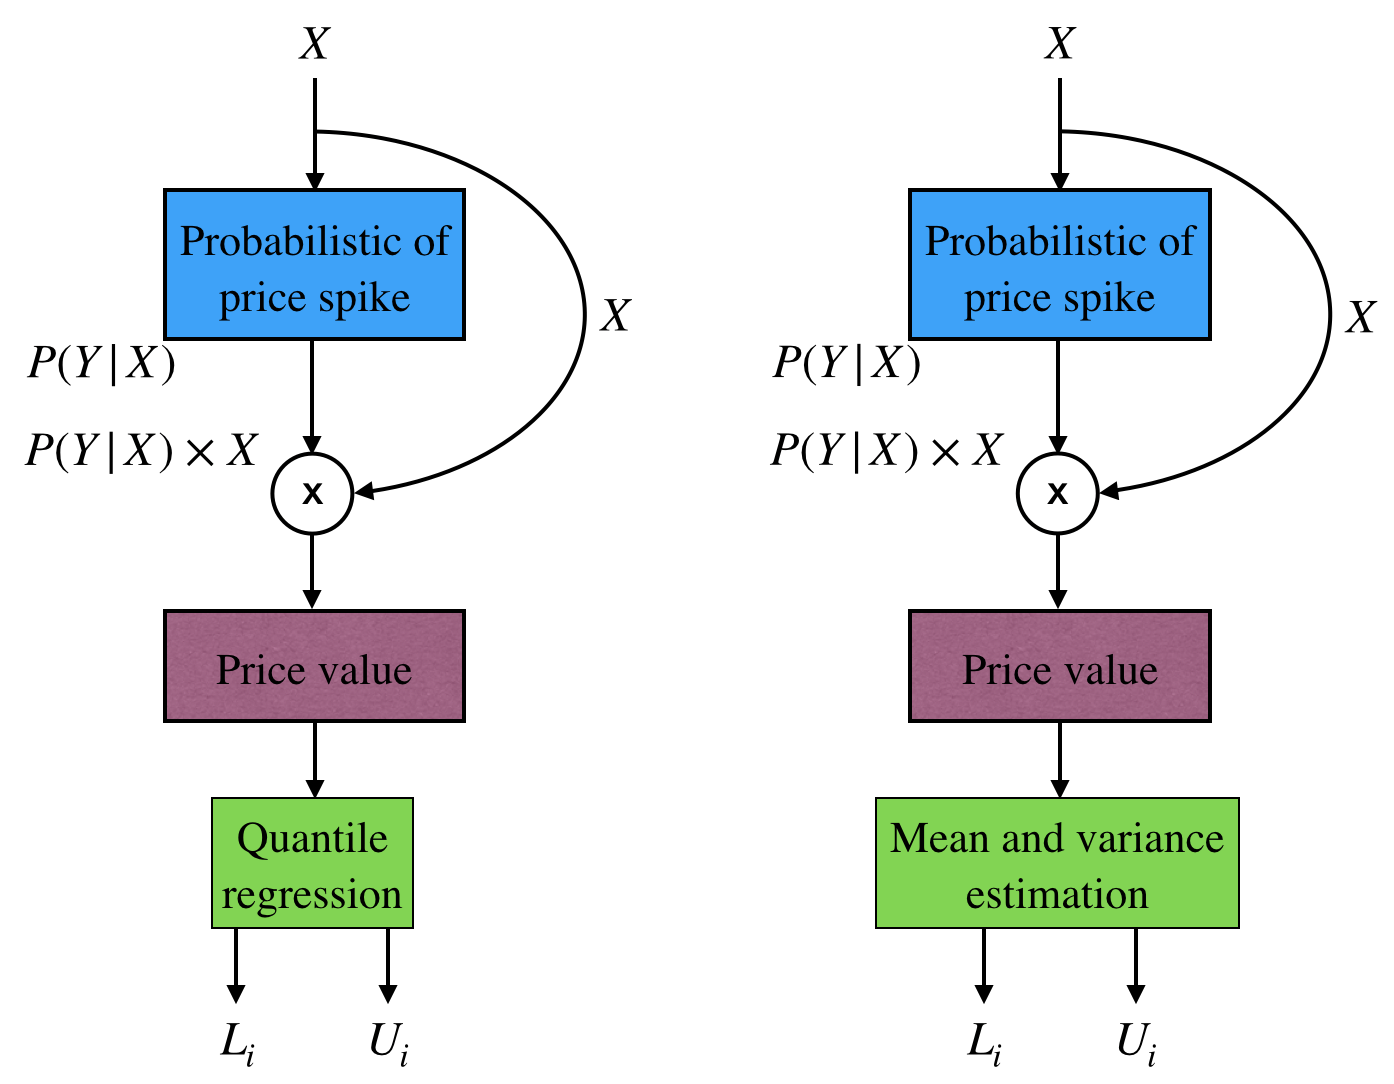
\includegraphics[width=12cm]{UB_LB_MV_PDRNN}
        \caption{The proposed ResNet models with LUBE (left) quantile regression and (right) mean and variance estimation.}
        \label{Fig:UB_LB_MV_PDRNN}
        \centering
      \end{figure}

      In brief, the proposed ResNet consists of two network layers.
      First is the classification layer of regular, high and spike prices probability.
      Second is the regression layer to produce electricity forecasting value.
      The input data is fed to second layers through short-cut paths.

    \subsection{The lower upper bound estimation}
      The lower upper bound estimation (LUBE) of interval electricity prices forecasting are formulated using two methods; quantile regression (QR), and mean and variance estimation (MV), respectively.
      Firstly, the QR method represents asymmetrical LUBE with relation with confidence level ($\alpha$) value from quantile function as express in Equation~\ref{eq.QR}.
      \begin{equation}
        [L_{i}, U_{i}]=
        \begin{cases}
        L_{i}=\int_{0}^{a} ppf(x) dx\\
        U_{i}=\int_{1-a}^{1} ppf(x) dx
        \end{cases}
        \label{eq.QR}
      \end{equation}
      The $L_{i}$ and $U_{i}$ are lower and upper bounds generated from quantile function $\int ppf(x) dx$ with given input $x$.

      Secondly, MV method represents symmetrical LUBE with relation with confidence level ($\alpha$) value from normal distribution function as express in Equation~\ref{eq.MV}.
      \begin{equation}
        [L_{i}, U_{i}]=
        \begin{cases}
          L_{i}=\bar{x} - z_{\alpha} \times \sqrt{\hat{\sigma}^2}\\
          U_{i}=\bar{x} + z_{\alpha} \times \sqrt{\hat{\sigma}^2}
        \end{cases}
        \label{eq.MV}
      \end{equation}
      where $\bar{x}$ and $\hat{\sigma}^2$ is mean and variance values generated from proposed forecasting model. $z_{\alpha}$ is critical value at confidence level $\alpha$.


      Figure~\ref{Fig:UB_LB_MV_PDRNN} illustrates a brief proposed probabilistic electricity prices forecasting model based on ResNet with quantile regression and mean and variance method or called ResNet-QR and ResNet-MV models.
      The set of load values, $X$, which is a total zonal load and a total system load as provided in GEFCom2014 provides.
      $P(Y|X)$ is a probability function generated from probabilistic of spike prices part, the first part of ResNet.
      The $L{i}$ and $U_{i}$ values are lower and upper bound of interval forecasting at time $i$.


      \subsection{Evaluation metrics}
        This section will descript evaluation metrics on accuracy and reliable point of view.
        In term of accuracy aspect, the forecasting results will be analyzed using pinball loss function.
        The Coverage Width-based Criterion (CWC) will take care of the reliability aspect.

        \subsubsection{Accuracy aspect}
          The widely used measurement of forecasting's accuracy is mean absolute error (MAE) which is the generalized and straightforward method.
          MAE work well of a point of forecasting (single value).
          However, this problem leads to the upper and lower bound of forecasting which it cooperates with a confidence value.
          Hence, general MAE is not satisfied in this case.
          The pinball loss function is proposed in \cite{Maciejowska2016}, also be the benchmark of this paper, which returns the values or called loss values that can be interpreted as the accuracy of mean and variance and quantile regression forecasting models.
          The pinball loss function is formulated in Equation~\ref{eq.pinball}.

          \begin{equation}
            L_{\tau}(y,z) =
            \begin{cases}
              (y-z)\tau & \text{if  $y>=z$} \\
              (z-y)(1-\tau) & \text{if  $z>y$}
            \end{cases}
            \label{eq.pinball}
          \end{equation}
          where $L_{\tau}(y,z)$ is pinball loss function at $\tau$ confidence level, $y$ is forecasted electricity prices and $z$ is actual electricty price.
          The final score of pinball loss function was computed as average $L_{\tau}$ across 24 hours for each task.
          The $\tau$ in this paper is 0.05, 0.10, 0.15, 0.20 and 0.25 which are represent 5$\%$, 10$\%$, 15$\%$, 20$\%$ and 25$\%$ confidence levels.
          The essential results of the pinball loss function are that the lower pinball loss, the more accurate forecasting model.

        \subsubsection{Reliability aspect}
        In term of reliability measurement, the performances of the forecasting model can ensure that the ranges of interval electricity prices forecasting are covering the observation values both quality and quantity.

        Firstly, the forecasting model can construct prediction intervals (PIs), upper and lower bound values, which able to cover the actual target values within the range. The number of covered actual target values over every target values is called prediction interval coverage probability (PICP).
        PICP can be mathematically stated as
        \begin{equation}
          \text{PICP} = \frac{1}{N} \sum_{i=1}^{N} C_{i}
          \label{eq.PICP}
        \end{equation}
        where
        \begin{equation}
          C_{i} =
          \begin{cases}
            1, & \text{if  $t_{i} \in [L_{i},U_{i}]$} \\
            0, & \text{if  $t_{i} \not\in [L_{i},U_{i}]$}
          \end{cases}
          \label{eq.Ci}
        \end{equation}
        where $N$ is the number of forecasted electricity price set, $t_{i}$ represents the actual electricity price, and $L_{i}$ and $U_{i}$ are lower and upper bounds of electricity price interval forecasting in hour $i$th, respestively.
        When the PIs can enclose all actual electricity price for all period, the PICP of the forecasting model is 1.
        The PICP is decreased when actual electricity prices lie outside the PIs and become 0 when none of the actual electricity prices lie outside the PIs.
        The PICP has a direct relationship with the width of PIs.
        Since the width of PIs is large, the PICP is higher.
        As a result of increasing of the PICP is achieved by extending the width of PIs.
        The PICP should be more significant than the nominal confidence level associated with the PIs.
        Secondly, the widths of PIs are too varied in each period.
        Therefore, it can be analyzed to averaged value as Mean PI Width (MPIW) \cite{Khosravi2010} as shown in equation~\ref{eq.MPIW}.

        \begin{equation}
          \text{MPIW} = \frac{1}{N} \sum_{i=1}^{N} (U_{i}-L_{i})
          \label{eq.MPIW}
        \end{equation}

        MPIW can be formed as a nominal value by the range of the underlying target, $R$.
        This new value is called NMPIW.
        NMPIW can be used to compare with results of other PIs forecasting model and different datasets.
        The $R$ in this paper is 10 $\$$/MWhr.

        \begin{equation}
          \text{NMPIW} = \frac{\text{MPIW}}{R}
          \label{eq.NMPIW}
        \end{equation}

        Both PICP and NMPIW, are representing the probability (actual electricity underlined prediction interval) and width of PIs, evaluate the quality of PIs from each aspect, respectively.
        The PICP and NMPIW can be combined into one index which represents a comprehensive assessment of PIs performances, both coverage probability, and width perspectives.
        The new index represents norminal width of PIs with penalties of low coverage probability as called Coverage Width-based Criterion (CWC) which is stated in Equation~\ref{eq.CWC-1}-\ref{eq.CWC-2}.

        \begin{equation}
          \text{CWC}=\text{NMPIW} \times (1+\gamma(\text{PICP})e^{(-\eta(\text{PICP}-\mu)})
          \label{eq.CWC-1}
        \end{equation}
        where
        \begin{equation}
          \gamma =
                \begin{cases}
                  0, \quad \text{PICP $\geq$ $\mu$} \\
                  1, \quad \text{PICP $<$ $\mu$} \\
                \end{cases}
          \label{eq.CWC-2}
        \end{equation}
        Where $\eta$ and $\mu$ are two hyperparameters controlling the location and amount of CWC jump.
        These measures can be readily determined based on the level of confidence associated with PIs.
        $\mu$ corresponds to the nominal confidence level associated with PIs and can be set to 1-$\alpha$.

        The CWC values are designed as the comparison between PICP and confidence level (1-$\alpha$)$\%$.
        If PICP is less than the confidence level, CWC value will be influenced by the exponential term of CWC.
        In the opposite site, CWC will be equal to NMPIW since $\gamma$ is eliminated when PICP is equal or larger than confidence level.

    \subsection{Data description}
      All data in this paper is provided in Global Energy Forecasting Competition 2014 (see \cite{Hong2016}).
      This competition aims to forecast 15 tasks of electricity prices in term of probabilistic distribution (in quantiles).
      Hourly data of locational marginal prices (LMP), zonal load forecast and system load forecast are provided.
      The participants receive historical data and forecast for next day electricity price.
      In total, the prices forecasting track involves about three years of locational marginal price, zonal and system load forecast.
      The summarized solution data set of 15 tasks is shown in Table~\ref{table:price_data_set}.
      \begin{table}[H]
        \begin{center}
        \caption{Summary of GEFCom2014 electricity prices forecasting tasks.}
        \begin{adjustbox}{width=\textwidth}
          \begin{tabular}{|c|c|c|c|c|c|c|}
            \hline
            Task & Day & Holiday & Season & Normal prices & High prices & Spike price\\
            \hline
            1 & Sun & Yes & Summer & 24 & - & -\\
            2 & Mon & No & Summer & 24 & - & -\\
            3 & Mon & No & Summer & 22 & 2 & -\\
            4 & Thu & No & Summer & 24 & - & -\\
            5 & Tue & No & Summer & 22 & 2 & -\\
            6 & Sat & Yes & Summer & 24 & - & -\\
            7 & Tue & No & Summer & 16 & 8 & -\\
            8 & Thu & No & Summer & 12 & 8 & 4\\
            9 & Fri & No & Summer & 13 & 6 & 5\\
            10 & Sat & Yes & Summer & 18 & 6 & -\\
            11 & Wed & No & Summer & 24 & - & -\\
            12 & Thu & No & Summer & 24 & - & -\\
            13 & Sat & Yes & Authumn & 24 & - & -\\
            14 & Sun & Yes & Authumn & 24 & - & -\\
            15 & Tue & No & Authumn & 15 & 9 & -\\
            \hline
          \end{tabular}
        \end{adjustbox}
        \label{table:price_data_set}
        \end{center}
      \end{table}

      The participation teams in GEFCom2014 perform electricity prices forecasting method i.e.; linear regression (IR)\cite{Dudek2016}, multilayer perceptron (MLP)\cite{Dudek2016},  multiple quantile regression\cite{Juban2016}, hybrid quantile regression average (QRA) with pre-and-post processes\cite{Maciejowska2016}.

  \section{Results}
    In the accuracy point of view, the results were evaluated with pinball loss function and summarized in Table~\ref{table:result_pinball}.
    The outcomes of the benchmarks and proposed ResNet electricity prices forecasting models indicate that some tasks involve more uncertainty than others day.
    Benchmark-1, provided by GEFCom2014 data, is shallow accuracy level, a high value of pinball loss score, in Task7-12 and 15.
    Benchmark-2 included mixed of ARX model, pre-filtering process, quantile estimation, and post-processing in order to acquire more accuracy of competition task.
    The difficulty of forecasting in the mentioned task lied in high forecasting zonal load.
    It was evident that high forecasted load may trigger an electricity spike price.
    The MLP-MV and MPL-QR models were developed to illustrate a simple forecasting model without spike prices prediction.
    The similar work of this approach is found in \cite{Dudek2016}.
    The MLP models are unsuitable for task 8-9 since loss score is very high.
    However, in the task without spike price, the models perform quite acceptable comparing to Benchmark-1 model.

    The next result we will discuss is that the proposed ResNet generated upper and lower bound values using quantile regression and mean-variance method.
    Both ResNet-MV and ResNet-QR model performed excellent work and provide lower losses score comparing to Benchmark-1, MLP-MV, and MLP-QR.
    Besides, both proposed models also provided similar losses score with Benchmark-2 \cite{Maciejowska2016} as seen in Table~\ref{table:result_pinball}.

    \begin{table}[H]
      \caption{The results of probabilistic electricity prices forecasting compared to benchmarks.}
      \begin{adjustbox}{width=\textwidth}
      \begin{threeparttable}
        \begin{center}
          \begin{tabular}{ccccccc}
            \hline
            Method & Task 4 & Task 5& Task 6 & Task 7& Task 8 & Task 9\\
            \hline
            Benchmark-1 \tnote{a} & 4.03 & 7.97 & 5.70 & 22.32 & 38.34 & 44.23 \\
            Benchmark-2 \tnote{b} & 1.00 & 1.82 & 1.19 & 2.82 & 7.56 & 4.21 \\
            \hline
            MLP-MV & 4.19 & 4.33 & 4.18 & 10.48 & 31.57 & 33.35 \\
            MLP-QR & 2.57 & 4.03 & 2.55 & 12.96 & 34.76 & 36.24 \\
            ResNet-MV& 2.45 & 3.36 & 2.39 & 5.79 & 8.79 & 6.95 \\
            ResNet-QR& 2.11& 3.47& 1.93 & 6.14 & 9.41 & 7.63 \\
            \hline
            \\
            \hline
            Method & Task 10 & Task 11& Task 12 & Task 13 & Task 14 & Task 15\\
            \hline
            Benchmark-1 \tnote{a} &  18.22 & 31.57 & 42.95 & 2.86 & 3.20 & 22.38\\
            Benchmark-2 \tnote{b} &  2.60 & 1.05 & 1.24 & 4.06 & 1.08 & 3.07 \\
            \hline
            MLP-MV &  6.28 & 4.28 & 4.25 & 4.06 & 4.05 & 13.02\\
            MLP-QR &  8.83 & 2.51 & 2.49 & 2.47 & 2.62 & 16.81\\
            ResNet-MV & 5.80 & 2.41 & 2.41 & 2.34 & 2.43 & 11.02 \\
            ResNet-QR & 6.38 & 1.88 & 1.91 & 2.01 & 2.22 &11.70 \\
            \hline
          \end{tabular}
            \begin{tablenotes}
              Notes: The numbers are calculated according to the pinball loss function
              \item[a] benchmark data provided by GEFCom2014.
              \item[b] hybrid model extending the Quantile Regression Averaging (QRA) approach provided in \cite{Maciejowska2016}.
            \end{tablenotes}
        \end{center}
      \end{threeparttable}
      \end{adjustbox}
      \label{table:result_pinball}
    \end{table}

    In Figure~\ref{Fig:compare_spike_and_non_spike_model}, the filled area represent interval prediction of MLP-QR and ResNet-QR with 5$\%$ confidence level.
    In cleary comparison between MLP and ResNet models, Figure~\ref{Fig:compare_spike_and_non_spike_model} shows the area covered by upper and lower quantile value, with 5$\%$ confidence level, generated by those models.
    The ResNet-QR model can forecast the high and spike prices over task 9 data. On the other hand, MLP-QR model is unsuitable for handling prices spike prediction.
    \begin{figure}[H]
      \centering
      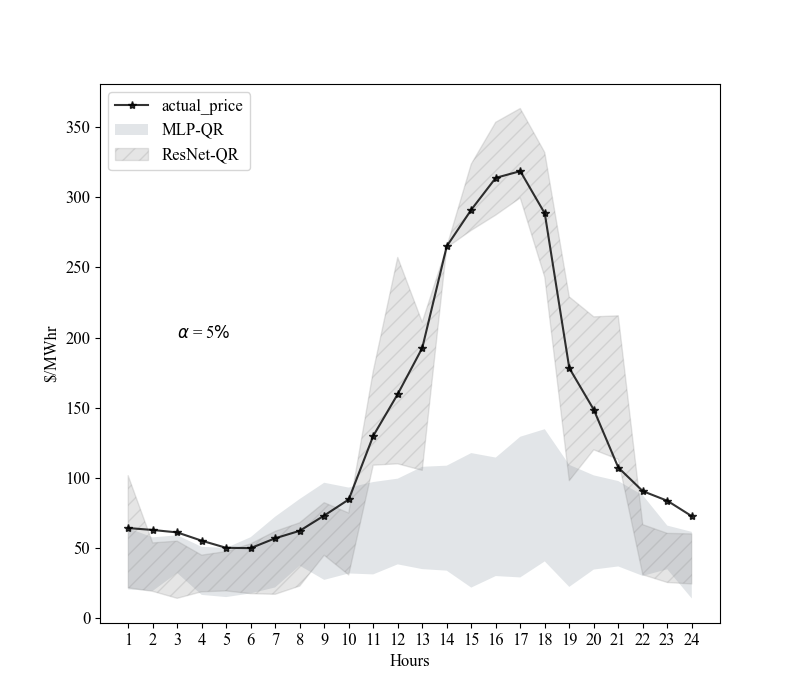
\includegraphics[width=12cm]{Task_9-compare_between_non-spike_and_spike}
      \caption{The task 9 results of non-spike price, MLP-QR, forecasting model and spike price, ResNet-QR, forecasting model with quantile regression method with 5$\%$ confidence level ($\alpha$).}
      \label{Fig:compare_spike_and_non_spike_model}
    \end{figure}

    Figure~\ref{Fig:all_task_QR_005} presents the overall results of interval electricity prices prediction of ResNet-QR model with 5$\%$ confidence level.
    In task 4, 5, 6, 11, 12, 13 and 14, there is no number of spike prices in the system.
    The proposed ResNet-QR can predict lower and upper electricity prices bound and cover the fluctuated real prices in these tasks.
    Furthermore, the proposed ResNet-QR model has the capability of interval prediction of spike prices occurred in task 7, 8, 9 and 10.

    \begin{figure}[H]
      \centering
      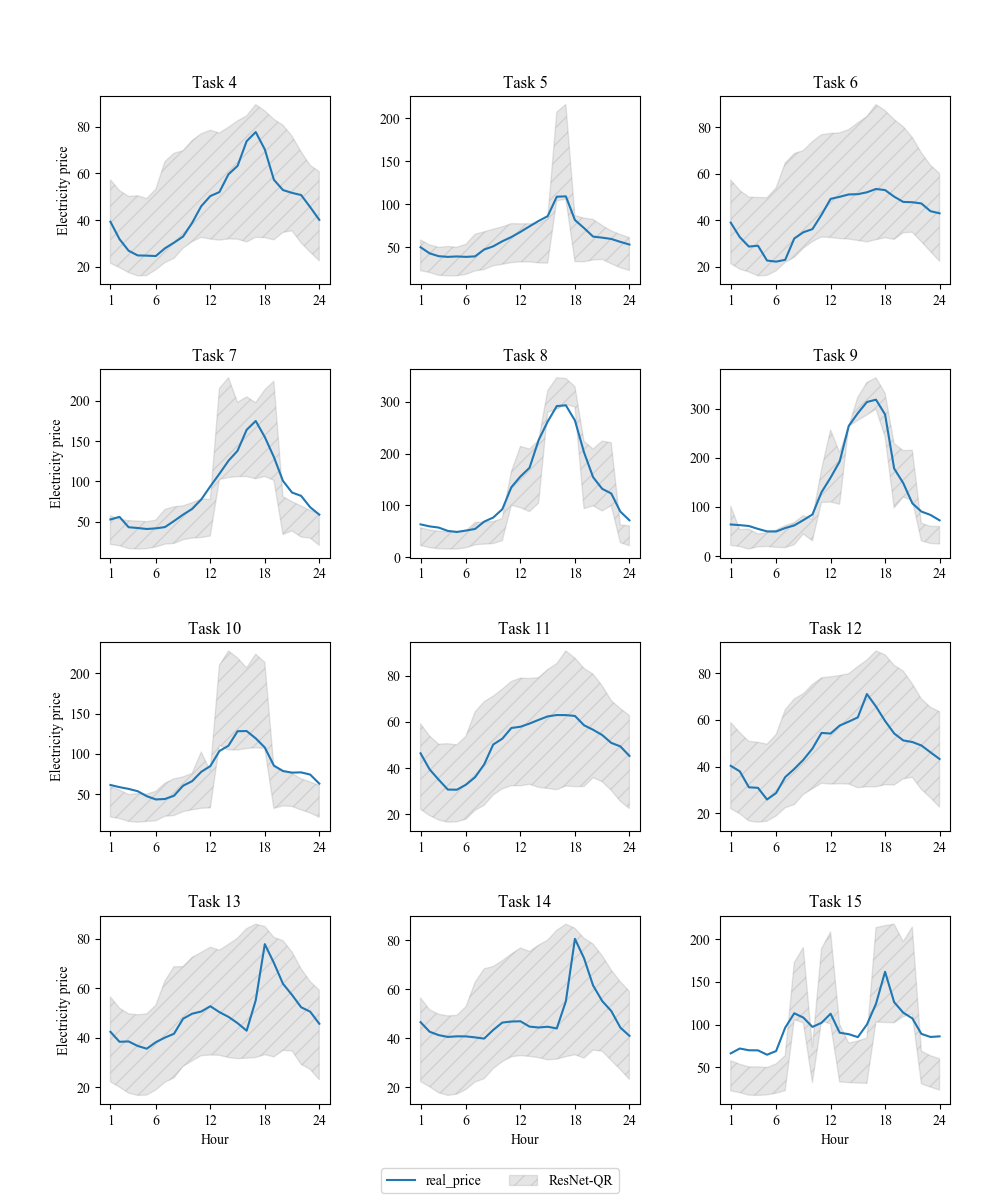
\includegraphics[width=15cm]{All_task_with_spike_price_QR_005}
      \caption{The results of ResNet-QR with 5$\%$ confidence level in task 4-15.}
      \label{Fig:all_task_QR_005}
    \end{figure}

    Second, we will discuss more on the effect of confidence levels ($\alpha$) to the reliability aspect of the proposed model here.
    All CWC values are analyzed using distribution characteristic in each model at differenced confidence level (5$\%$, 10$\%$, 15$\%$, 20$\%$ and 25$\%$).
    The Figure~\ref{Fig:CWC} illustrates all CWC value where bold line represents averaged CWC values, of all task, of particular model and confidence level.
    The boxes contain 50$\%$ (at quantile 25$\%$ to 75$\%$) of result CWC values.
    The top and bottom whiskers show the highest and lowest CWC values in each box.
    Since CWC value represents both coverage probability and width perspective, the lower CWC value represents higher reliability.
    The Figure~\ref{Fig:CWC} shows that while increasing confidence level, the models could perform better in CWC perspective.
    The averaged CWC value could drop below 15 while increasing confidence level up to 15 $\%$ for ResNet models.
    Moreover, the quantile regression method provides higher reliability aspect than the mean-variance method as seen in Figure~\ref{Fig:CWC}.

    \begin{figure}[H]
      \centering
      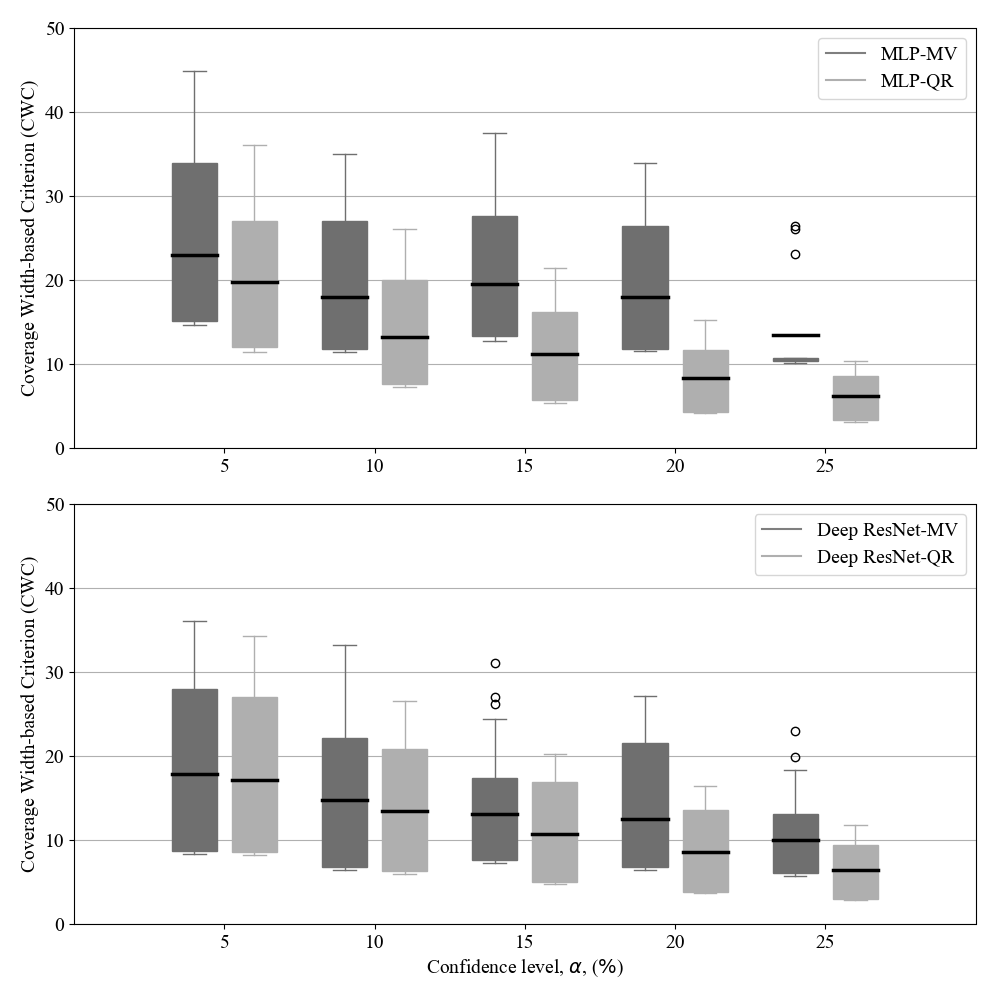
\includegraphics[width=12cm]{boxcompare_MV-QR}
      \caption{The results of the reliability aspect are represented in CWC values (upper) MLP model, (lower) ResNet model.}
      \label{Fig:CWC}
    \end{figure}

    In summary, we have already considered both accuracy and reliability aspects of proposed ResNet models through pinball losses score and CWC values, respectively.
    The MLP models have low performance on task 8 and 9 where spike prices occurred in the tasks.
    Besides, the MLP models could not predict the range of electricity prices during the high forecasted system and zonal load.
    On the other hand, ResNet model can cover forecast interval of electricity prices in mostly tasks where MLP could not.
    Lastly, the quantile regression method performs similar pinball loss score results comparing to mean and variance estimation method in accuracy aspect.
    However, the quantile regression method provider better CWC values.
    Consequently, the proposed ResNet with quantile regression could perform best in both accuracy and reliability aspect of the forecasting model.

  \section{Conclusions}
  This paper proposes a novel application of Residual Neural Network (ResNet) based approach to probabilistic electricity prices forecasting in term of Quantile Regression and Mean and Variance Estimation as lower and upper bound estimation (LUBE).
  The proposed models are demonstrated with GEFCom2014's electricity prices forecasting tasks. The results of proposed and benchmark models are evaluated in accuracy and reliability point of view through pinball loss function and Coverage Width-based Criterion (CWC).
  The two significant observation results were:
  (i) the electricity prices forecasting model, the proposed ResNet model, with high and spike prices prediction capability can perform better than a simple plain model, MLP model,
  (ii) the lower and upper bound of interval prediction using the asymmetrical model (quantile regression) could perform better than the symmetrical model (mean and variance estimation) since it could reduce the width of interval prediction.
  To improve the quality of the forecasting model in future studies, the proposed ResNet model should cooperate with other LUBE methods.
  The other LUBE has its characteristics which may provide better CWC values.
  The second way to improve the performance of the proposed ResNet forecasting model is to increase the layers within the model.
  The fined tuning forecasting deep ResNet model may perform an excellent job on electricity prices forecasting tasks.

  \section*{References}
  \bibliography{mybibfile}
\end{document}
